\documentclass[10pt]{article}
\usepackage{fullpage}
\usepackage{graphicx}
\usepackage{amsmath}

\author{Mirko van de Hoef}
\title{Deriving equations of motions of a double pendulum on a cart using the Lagrangian}
\date{\today}
\graphicspath{
    {img/}
}

\begin{document}

    \maketitle

    \section{Introduction}
    This file is made to document the simulation of a double pendulum on a cart using lagrangian mechanics. 
    In this file a double pendulum on a cart will be discussed.

    \section{The system}
    \begin{figure}{t}
        \centering
        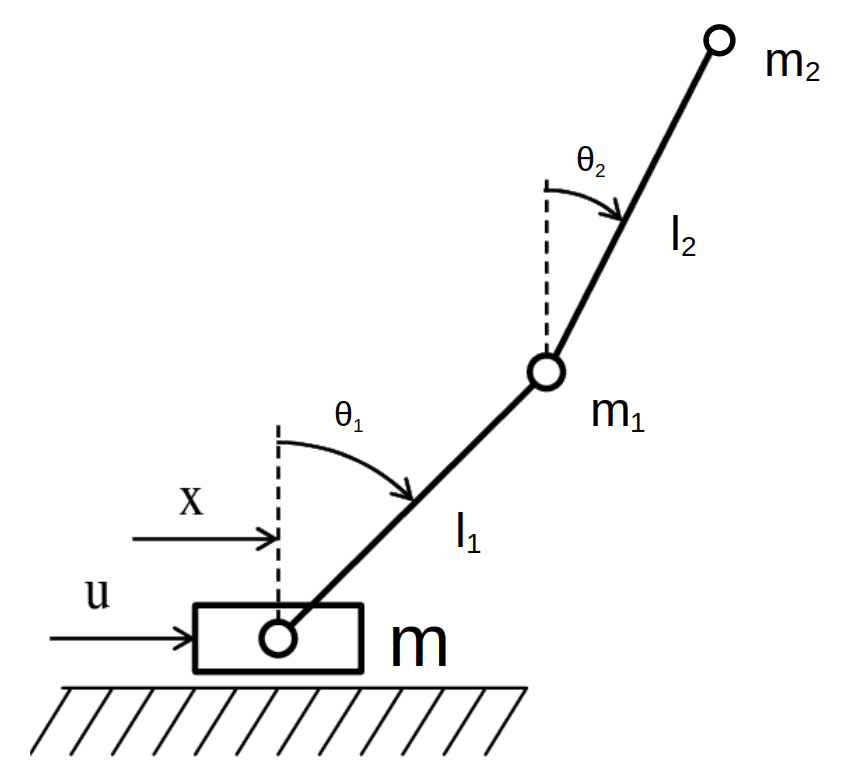
\includegraphics[width=5cm]{post-aRippol-02-pendulum_notations.png}
        \caption{The pendulum}
        \label{fig:system}
    \end{figure}
    
    Where in figure \ref{fig:system}: \\
    \begin{tabular}{@{}l l l@{}}
        & $M$: & Mass of the cart  [kg] \\
        & $m_1$: & Mass of the first pendulum  [kg] \\
        & $m_2$: & Mass of the second pendulum  [kg] \\
        & $\theta_1$: & Degrees first pendulum in reference to the cart [rad] \\
        & $\theta_2$: & Degrees second pendulum in reference to the cart [rad] \\
        & $\ell_1$: & Length of the first pendulum [m] \\
        & $\ell_2$: & Length of the second pendulum [m] \\
        & $x_c$: & Position of the cart [m] \\
    \end{tabular}
    

    \section{Lagrangian}
    Let the position and velocity of the pendulum be
    \begin{equation*}
    \begin{aligned}
        x_1 &= \ell_1 \sin(\theta_1) + x_c                                    & & \qquad \qquad & \dot x_1 &= \ell_1 \dot \theta_1 \cos(\theta_1) + \dot x \\
        y_1 &= -\ell_1 \cos(\theta_1)                                         & &  \quad \qquad & \dot y_1 &= \ell_1 \dot \theta_1 \sin(\theta_1)  \\
        x_2 &= \ell_1 \sin(\theta_1) + \ell_2 \sin(\theta_2) + x_c            & & \qquad \qquad & \dot x_2 &= \ell_1 \theta_1 \cos(\theta_1) + \ell_2 \dot \theta_2 \cos(\theta_2) + \dot x \\
        y_2 &= -\ell_1 \cos(\theta_1) - \ell_2 \cos(\theta_2)                 & &  \quad \qquad & \dot y_2 &= \ell_1 \dot \theta_1 \sin(\theta_1) + \ell_2 \dot \theta_2 \sin(\theta_2)  \\
    \end{aligned}
    \end{equation*}
    

    To derive the equations of motion, the Lagrangian (\ref{eq:lagrangian}) will be used.
    First, $T$, the kinetic energy of the system will be calculated.

    \begin{equation} \label{eq:lagrangian}
        \mathcal{L} = T - V
    \end{equation}

    \begin{equation}
        \begin{aligned} \label{eq:kinetic}
            T &= \frac{1}{2}  M  \dot x^2 + \frac{1}{2}  m (\dot x_s^2 + \dot y_s^2) \\
            T &= \frac{1}{2}  M  \dot x^2 + \frac{1}{2} m((\dot x + \ell  \dot \theta  cos(\theta))^2 + (\ell  \dot \theta  sin(\theta))^2) \\
            T &= \frac{1}{2}  M  \dot x^2 + \frac{1}{2}  m(\dot x^2 + 2 \dot x  \ell  \dot \theta  cos(\theta) + \ell^2  \dot \theta^2 cos(\theta)^2 + \ell^2  \dot \theta^2  sin(\theta)^2) \\
            T &= \frac{1}{2}  M  \dot x^2 + \frac{1}{2} m(\dot x^2 + 2 \dot x \ell \dot \theta cos(\theta) + \ell^2 \dot \theta^2) \\
            T &= \frac{1}{2}(M + m) \dot x^2 + \frac{1}{2}m(2 \dot x \ell \dot \theta cos(\theta) + \ell^2 \dot \theta^2) \\
            T &= \frac{1}{2}(M + m) \dot x^2 + m \dot x \ell \dot \theta cos(\theta) + \frac{1}{2}m \ell^2 \dot \theta^2 
        \end{aligned}
    \end{equation}

    Then, for $V$, the potential energy of the system

    \begin{equation} \label{eq:potential}
        \begin{aligned}
        V &= m_1gy_1 + m_2gy_2     \\
        V &= -m_1g\ell_1\cos(\theta_1) - m_2g\ell_2\cos(\theta_2)\\
        V &= -(m_1+m_2)g\ell_1\cos(\theta_1) - m_2g\ell_2\cos(\theta_2)
        \end{aligned}
    \end{equation}
    
    Lastly, using (\ref{eq:kinetic}) and (\ref{eq:potential}) the 
    Lagrangian, $\mathcal{L}$, can be formulated
    
    \begin{equation} \label{eq:lagrangian_full}
        \begin{aligned}
            \mathcal{L} = & \frac{1}{2}(M + m_1) \dot x_c^2 \\
            & + \frac{1}{2}(m_1 + m_2)\ell_1^2\dot\theta_1^2 \\
            & + \frac{1}{2} m_2 \left(2\ell_1\ell_2 \dot\theta_1 \dot\theta_2 \cos(\theta_1 - \theta_2) + \ell_2^2\dot\theta_2^2 + 2\dot x_c(\ell_1 \dot \theta_1 \cos(\theta_1) + \ell_2 \dot \theta_2 \cos(\theta_2))\right) \\
            & + (m_1 + m_2)g\ell_1\cos(\theta_1) - m_2g\ell_2\cos(\theta_2)
        \end{aligned}
    \end{equation}
    

    \pagebreak
    \section{Solve for $\ddot \theta$}

    Using the Lagrangian equation (\ref{eq:lagrangian_eq})
    \begin{equation} \label{eq:lagrangian_eq}
        \frac{d}{dt} \left(\frac{\partial \mathcal{L}}{\partial \dot q} \right) = 
        \frac{\partial \mathcal{L}}{\partial q}
    \end{equation}

    Substituting (\ref{eq:lagrangian_full}) in equation (\ref{eq:lagrangian_eq}) and solving for $\theta_1$ gives:

    \begin{equation} \label{eq: lagrange Step1}
        \frac{\partial \mathcal{L}}{\partial \dot\theta_1} = 
         (m_1 + m_2)\ell_1^2\dot\theta_1 + m_2\ell_1\ell_2\dot\theta_2\cos(\theta_1 - \theta_2) + m_2\dot x_c\ell_1\cos(\theta_1)
    \end{equation}

    \begin{equation} \label{eq: lagrange Step2}
        \begin{aligned}
        \frac{d}{dt} \left(\frac{\partial \mathcal{L}}{\partial \dot\theta_1}\right) =& 
         (m_1 + m_2)\ell_1^2\ddot\theta_1   +   m_2\ell_1\ell_2\ddot\theta_2\cos(\theta_1 - \theta_2)  -m_2\ell_1\ell_2\dot\theta_2\sin(\theta_1-\theta_2)(\dot\theta_1 - \dot\theta_2) \\
           & +   m_2\ddot x_c\ell_1\cos(\theta_1) - m_2 \dot x_c\ell_1\sin(\theta_1)\dot\theta_1
        \end{aligned}
    \end{equation}

    
    \begin{equation} \label{eq: lagrange Step3}
        \frac{\partial \mathcal{L}}{\partial\theta_1} = 
        m_2\ell_1\ell_2\dot\theta_1\dot\theta_2\sin(\theta_1-\theta_2) 
        -m_2\dot x_c\ell_1\dot\theta_1\sin(\theta_1)
        - (m_1 + m_2)g\ell_1\sin(\theta_1)
    \end{equation}

    Which give the following differential equation:

    \begin{equation}
        \begin{aligned}
            &(m_1 + m_2)\ell_1^2\ddot\theta_1   +   m_2\ell_1\ell_2\ddot\theta_2\cos(\theta_1 - \theta_2)  -m_2\ell_1\ell_2\dot\theta_2\sin(\theta_1-\theta_2)(\dot\theta_1 - \dot\theta_2)\\
            &+   m_2\ddot x_c\ell_1\cos(\theta_1) - m_2 \dot x_c\ell_1\sin(\theta_1)\dot\theta_1 - m_2\ell_1\ell_2\dot\theta_1\dot\theta_2\sin(\theta_1-\theta_2)\\ 
            &-m_2\dot x_c\ell_1\dot\theta_1\sin(\theta_1) - (m_1 + m_2)g\ell_1\sin(\theta_1) = 0
        \end{aligned}
    \end{equation}   


    Which simplifies to:

    \begin{equation}
        \begin{aligned}
            &(m_1 + m_2)\ell_1\ddot\theta_1   +   m_2\ell_2\ddot\theta_2\cos(\theta_1 - \theta_2)  -m_2\ell_2\dot\theta_2^2\sin(\theta_1-\theta_2)\\
            &+   m_2\ddot x_c\cos(\theta_1) - (m_1 + m_2)g\sin(\theta_1) = 0
        \end{aligned}
    \end{equation}  

    With the differential equation solved for $\ddot \theta_1$:
    \begin{equation}
        \begin{aligned}
            \frac{m_2\ell_2\ddot\theta_2\cos(\theta_1 - \theta_2)  -m_2\ell_2\dot\theta_2^2\sin(\theta_1-\theta_2)
            +   m_2\ddot x_c\cos(\theta_1) - (m_1 + m_2)g\sin(\theta_1)}{-(m_1 + m_2)\ell_1} = \ddot \theta_1
        \end{aligned}
    \end{equation}  
    
    
    \section{Solve for $\ddot x$}
\end{document}